\documentclass[12pt,a4paper]{article}

% ---- Packages ----
\usepackage[margin=2.5cm]{geometry}
\usepackage[T1]{fontenc}
\usepackage[utf8]{inputenc}
\usepackage{lmodern}
\usepackage{amsmath, amssymb}
\usepackage{graphicx}
\usepackage{booktabs}
\usepackage{hyperref}
\usepackage{caption}
\usepackage{subcaption}
\usepackage{xcolor}
\usepackage{parskip}
\usepackage{setspace}
\usepackage{float}
\usepackage{microtype}
\usepackage{eurosym}   % commande \euro pour le symbole €

\hypersetup{
  colorlinks=true,
  linkcolor=blue!60!black,
  citecolor=blue!60!black,
  urlcolor=blue!60!black
}

\setstretch{1.2}

% ---- Custom commands ----
\newcommand{\soc}{\mathrm{SoC}}
\newcommand{\eg}{e.g.,\ }
\newcommand{\ie}{i.e.,\ }

% ---- Title ----
\title{\textbf{Applying Monte Carlo Tree Search to\\Energy Management}}
\author{M2 Academic Project}
\date{2025--2026}

\begin{document}

\maketitle
\tableofcontents
\newpage

% ==========================================================================
\section{Introduction}
% ==========================================================================

In this project, we look at a simple but realistic problem: a power plant
produces electricity every hour and has to decide what to do with it. It can
\textbf{sell} it on the market right away, \textbf{store} it in a battery for
later, or \textbf{consume} it internally to avoid buying electricity from the
grid. The goal is to make the best sequence of decisions over a whole day (or
week) to maximize the total profit.

This might sound straightforward, but it is actually a hard combinatorial
problem. If we only allow three decisions per hour, there are already
$3^{24} \approx 2.8 \times 10^{11}$ possible sequences for a single day.
Trying all of them is completely out of reach. This is exactly why we use
\textbf{Monte Carlo Tree Search (MCTS)}: it is an algorithm that explores the
decision tree intelligently, focusing on the most promising branches, without
needing to look at everything.

The prices we use come from the French day-ahead electricity market
(EPEX SPOT), retrieved from \texttt{energy-charts.info} (Fraunhofer ISE,
CC BY 4.0). Solar production data comes from \texttt{ODRÉ / éCO2mix} (RTE,
open data). We first test our approach on synthetic data (where we can control
everything), then validate it on real French data.

% ==========================================================================
\section{Problem Formulation}
% ==========================================================================

\subsection{The decision problem}

We model the problem as a \textbf{Markov Decision Process (MDP)}. At each
hour $t \in \{0, 1, \dots, H-1\}$, the plant has a battery with some level of
charge called the \emph{State of Charge} $\soc_t \in [0, C]$, where $C$ is
the battery capacity. It also produces $p_t$ MWh of electricity, and the
market price is $\lambda_t$ \euro/MWh.

The \textbf{state} is the pair $(t, \soc_t)$. At each step, the plant picks
an \textbf{action} that decides how to split the produced energy:

\begin{itemize}
  \item \textbf{Sell}: inject energy into the market at price $\lambda_t$.
  \item \textbf{Store}: charge the battery (with charging efficiency
    $\eta_c$), to sell or use later.
  \item \textbf{Consume}: use the energy internally, avoiding the need to buy
    electricity at the \emph{avoidance price} $p_c$ (\eg\ a retail tariff).
\end{itemize}

The plant never \emph{buys} from the market: it can only dispatch what it
produces or what is already in the battery. Storage simply shifts the timing
of how the plant's own energy is used.

The \textbf{reward} at step $t$ is:
\begin{equation}
  r_t = e_{\mathrm{sold},t} \cdot \lambda_t
      + e_{\mathrm{consumed},t} \cdot p_{c,t}
\end{equation}
where $e_{\mathrm{sold},t}$ and $e_{\mathrm{consumed},t}$ are the amounts
sold and consumed, respectively. The total profit is
$R = \sum_{t=0}^{H-1} r_t$ (no discounting).

\subsection{Battery dynamics}

When the plant decides to charge at a requested rate $u \geq 0$:
\begin{align}
  c &= \min\!\bigl(u,\; u_{\max},\; p_t,\; (C - \soc_t)/\eta_c\bigr) \\
  \soc_{t+1} &= \soc_t + \eta_c \cdot c \\
  e_{\mathrm{out},t} &= p_t - c
\end{align}
The charge is limited by the maximum charge rate $u_{\max}$, the production,
and the available battery space. When discharging at requested rate
$u_{\mathrm{req}} \geq 0$:
\begin{align}
  d &= \min\!\bigl(u_{\mathrm{req}},\; d_{\max},\; \soc_t\bigr) \\
  \soc_{t+1} &= \soc_t - d \\
  e_{\mathrm{out},t} &= p_t + \eta_d \cdot d
\end{align}
The discharge is limited by the maximum discharge rate $d_{\max}$ and the
current battery level. In both cases, $\soc_{t+1}$ is clipped to $[0, C]$.

\subsection{Action spaces}

We implemented two ways of defining actions:

\paragraph{Simple-3 mode.} The three literal actions from the problem
statement: SELL (discharge fully, sell everything), STORE (charge at maximum
rate, sell the surplus), CONSUME (serve the internal demand first, sell the
rest). This gives exactly the $3^H$ tree mentioned in the introduction.

\paragraph{Grid mode (default).} The action is a storage flow $u$ chosen from
a grid of $n$ values symmetric around zero ($n = 11$ by default). The split
between selling and consuming the dispatched energy is resolved by
\emph{dominance}: since this split does not affect the battery, it has no
future consequence and the optimal choice is immediate (consume first if
$p_c > \lambda_t$, up to demand, sell the rest). This keeps only the
non-trivial sequential decision — storage — in the action space, and gives an
even larger search tree: $11^{48} \approx 10^{50}$ for a two-day horizon.

% ==========================================================================
\section{Reference Strategies}
% ==========================================================================

To measure how well MCTS does, we compare it against several baselines.

\paragraph{Always-sell.} Sell everything at every step, never use the
battery. This is the zero-effort strategy and gives the lowest bar.

\paragraph{Greedy-myopic.} At each step, pick the action that maximizes the
\emph{immediate} reward. It never stores, because storing gives zero reward
right now. When there is no consumption channel, this makes it identical to
always-sell. When consumption is active, it can differ slightly: during
negative-price hours, consuming the energy internally (valued at the positive
avoidance price) beats selling it, so the greedy strategy consumes instead.
Either way, it shows the cost of ignoring the future value of the battery.

\paragraph{Price-threshold.} If the current price is above the median price,
discharge and sell at maximum rate; otherwise, charge at maximum rate. This is
the classic arbitrage heuristic: buy low, sell high.

\paragraph{Random.} Pick actions uniformly at random. This is the absolute
floor.

\paragraph{Dynamic Programming (DP).} The key reference. We solve the MDP
\emph{exactly} by backward induction on a discretized grid of $\soc$ values
(linear interpolation between grid points). This gives the
\textbf{theoretical optimum} under perfect information: no causal strategy can
do better. We use it as the 100\% mark.

\vspace{0.5em}
The metric we use throughout is the \textbf{arbitrage gain}:
\begin{equation}
  \text{gain} = \frac{\text{profit} - \text{profit}_{\text{no-storage}}}
                     {\text{profit}_{\text{DP}} - \text{profit}_{\text{no-storage}}}
                \times 100\%
\end{equation}
This tells us what fraction of the storage value a strategy captures.
``No storage'' scores 0\%; the DP optimum scores 100\%.

% ==========================================================================
\section{Monte Carlo Tree Search}
% ==========================================================================

\subsection{Overview}

MCTS is a planning algorithm that builds a search tree incrementally. It does
not need a closed-form solution: it only needs a \emph{simulator} (the ability
to simulate what happens when you take an action from a given state). Each
iteration of MCTS has four phases.

\subsection{The four phases}

\paragraph{1. Selection.} Start at the root node (the current state). Use the
\textbf{UCT formula} to pick which child to visit, and descend the tree until
you reach a node that has not been fully expanded yet:
\begin{equation}
  \text{UCT score}(a) = \underbrace{\frac{Q(a) - Q_{\min}}{Q_{\max} - Q_{\min}}}_{\text{exploitation}}
    + c \cdot \underbrace{\sqrt{\frac{\ln N_{\text{parent}}}{N(a)}}}_{\text{exploration}}
\end{equation}
where $Q(a)$ is the estimated value of action $a$, $N(a)$ is how many times
it has been visited, and $c$ is an exploration constant. The normalization
$[Q_{\min}, Q_{\max}] \to [0,1]$ makes the formula robust to the scale of
rewards (which can range from hundreds to millions of euros depending on the
instance).

\paragraph{2. Expansion.} Add one new child node for an action that has not
been tried yet from the selected node.

\paragraph{3. Simulation (rollout).} From the new node, simulate a complete
episode until the end of the horizon by following a \emph{rollout policy}.
This gives an estimate of the future reward. Two rollout policies are used:
\begin{itemize}
  \item \textbf{Random rollout}: pick actions uniformly at random.
  \item \textbf{Informed rollout}: use the price-threshold heuristic.
\end{itemize}

\paragraph{4. Backpropagation.} Walk back up the tree and update the visit
counts $N$ and cumulative returns $W$ of every node along the path. The
estimated value of a node is $W/N$.

\subsection{Rolling-horizon planning}

We use MCTS as a \textbf{rolling-horizon planner}: at each real time step $t$,
we build a fresh tree from the current state $(t, \soc_t)$, run the
simulations, pick the most-visited action, execute it, and move to $t+1$.
This is sometimes called Model Predictive Control (MPC). It means MCTS acts as
a \emph{policy} (a function from state to action) rather than a one-shot plan.

\subsection{Implementation details}

One subtle bug worth mentioning: when a node is at the last time step $H$, it
is a terminal node and returns 0. Without incrementing its visit counter, all
such terminal children have $N=1$, and the ``most-visited'' criterion becomes
arbitrary. We fixed this by counting terminal node visits and breaking ties by
estimated value. This bug was caught by our unit tests.

% ==========================================================================
\section{Experimental Results: Deterministic Setting}
% ==========================================================================

\subsection{Setup}

We use 48 hours of synthetic data: prices follow a realistic ``duck curve''
pattern (low at midday due to solar, peaks at 8 am and 7 pm), production is a
solar bell curve centered at noon, and internal demand has a small evening
peak. The battery has capacity 120\,MWh, charge/discharge rates of
30\,MW, and efficiencies $\eta_c = \eta_d = 0.95$. The avoidance price is
70\,\euro/MWh (corresponding to a retail tariff above the average spot price).

\subsection{Comparison of strategies}

Table~\ref{tab:det_results} shows the results for 5 random seeds (MCTS),
1000 simulations per time step.

\begin{table}[H]
  \centering
  \caption{Comparison of strategies on 48-hour synthetic data.
           Arbitrage gain = fraction of storage value captured
           (0\% = no storage, 100\% = DP optimum).
           MCTS results: mean $\pm$ std over 5 seeds.}
  \label{tab:det_results}
  \begin{tabular}{lrrr}
    \toprule
    Strategy & Profit & \% of optimum & \% arbitrage gain \\
    \midrule
    Random                     & 52\,245   & 89.0\% &  11.6\% \\
    No storage / Greedy-myopic & 51\,398   & 87.5\% &   0.0\% \\
    Price threshold            & 57\,627   & 98.1\% &  85.1\% \\
    MCTS, random rollout       & $55\,700 \pm 151$ & 94.9\% & 58.8\% \\
    \textbf{MCTS, informed rollout} & $\mathbf{58\,470 \pm 5}$ & \textbf{99.6\%} & \textbf{96.6\%} \\
    DP Optimum (upper bound)   & 58\,717   & 100\% & 100\% \\
    \bottomrule
  \end{tabular}
\end{table}

Several observations:
\begin{itemize}
  \item The greedy-myopic strategy performs just like no storage: ignoring
    the future completely destroys the value of the battery.
  \item The price-threshold heuristic is already strong (85.1\% arbitrage),
    but it uses a fixed rule and does not adapt.
  \item MCTS with a random rollout captures only 58.8\%: random continuations
    rarely ``use'' the stored energy at the right time, so the tree
    underestimates the value of charging.
  \item \textbf{MCTS with an informed rollout reaches 96.6\%} of the storage
    value, very close to the theoretical optimum, with almost no variance
    across seeds ($\pm 0.1\%$).
\end{itemize}

\paragraph{Simple-3 mode.} We also ran the literal three-action version from
the problem statement ($3^{48}$ search tree). MCTS with the informed rollout
achieves 95.7\% of arbitrage in that space, confirming the result holds
regardless of how the action space is defined.

Figure~\ref{fig:synth_traj} shows the data and the storage trajectories.
MCTS with an informed rollout closely tracks the DP-optimal battery use:
charging during the low-price midday hours and discharging into the evening
peaks.

\begin{figure}[H]
  \centering
  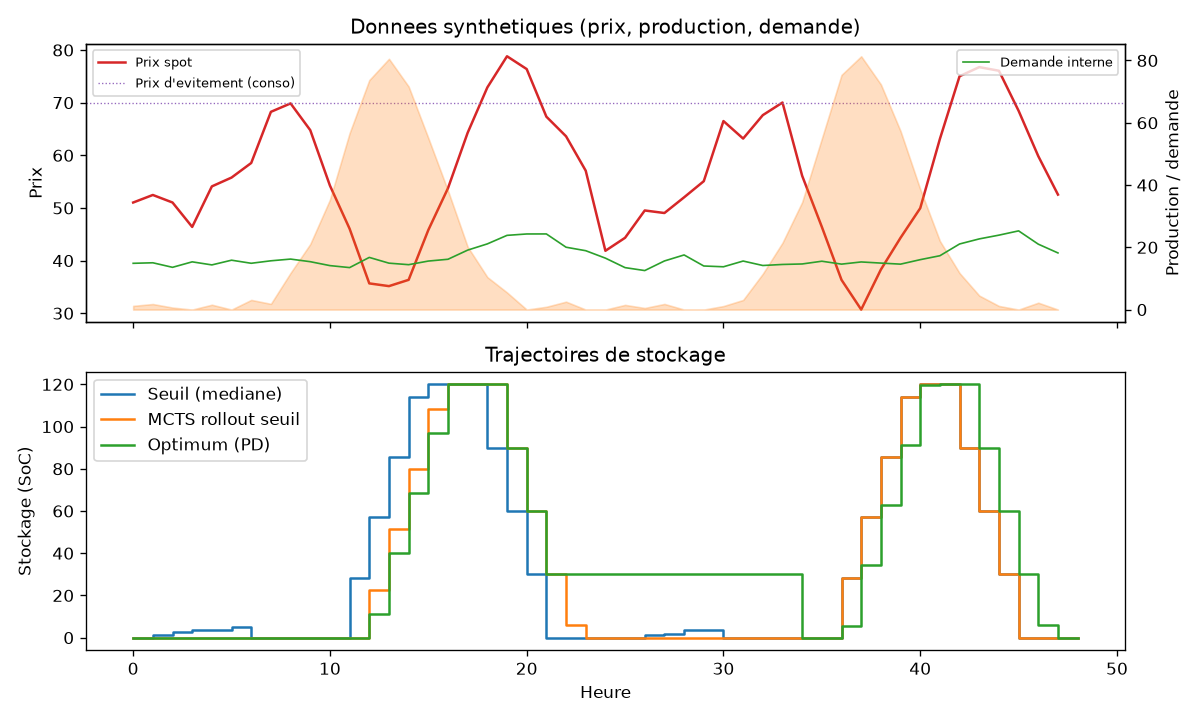
\includegraphics[width=\textwidth]{../figures/comparaison.png}
  \caption{Synthetic data (48 h). Top: spot price, solar production, internal
           demand, and the avoidance price line. Bottom: storage trajectories
           of the threshold heuristic, MCTS (informed rollout), and the DP
           optimum. MCTS follows the optimal charge/discharge pattern.}
  \label{fig:synth_traj}
\end{figure}

\subsection{Timing}

Table~\ref{tab:timing} reports the compute cost, measured on an AMD Ryzen CPU
(Python 3.12). Two things stand out. First, on this small deterministic
instance, dynamic programming is actually \emph{cheap} (0.35\,s for the whole
episode), and MCTS only matches it at a low budget of $\sim$100 simulations
per step. So MCTS is not faster than DP here. Second, MCTS cost grows roughly
linearly with the simulation budget.

\begin{table}[H]
  \centering
  \caption{Compute time on the 48-hour instance (11 actions), averaged over
           3 runs. MCTS uses the informed rollout. DP solves the whole episode
           at once; MCTS re-plans at every step.}
  \label{tab:timing}
  \begin{tabular}{lrr}
    \toprule
    Method & Time / step & Time / episode (48 steps) \\
    \midrule
    DP optimum ($n_{\soc}=241$) & --- & 0.35\,s \\
    MCTS, 100 sims/step  & 0.009\,s & 0.22\,s \\
    MCTS, 300 sims/step  & 0.027\,s & 0.69\,s \\
    MCTS, 1000 sims/step & 0.096\,s & 2.58\,s \\
    \bottomrule
  \end{tabular}
\end{table}

The real reason to prefer MCTS is not raw speed on this toy instance: DP wins
here precisely because the state is small and fully known. DP needs an
explicit, discretized state and perfect information. Its cost explodes when
the state grows (the ``curse of dimensionality''), and it cannot be used at
all when we only have a simulator. MCTS keeps working in both cases. The next
subsection makes this concrete.

\subsection{When MCTS becomes faster: scaling with the state size}

To show \emph{where} MCTS actually wins on speed, we make the state bigger.
Instead of one battery, we give the plant $B$ batteries with \emph{different}
efficiencies (so we genuinely have to track each one — they cannot be merged).
The state becomes the vector of $B$ charge levels. Crucially, we keep the
action space small (charge or discharge one chosen battery, $2B+1$ actions),
so only the \emph{state} dimension grows.

The cost of DP on a grid is $O(H \cdot n_{\soc}^{B} \cdot n_{\text{actions}})$:
the $n_{\soc}^{B}$ term grows exponentially with the number of batteries. MCTS,
on the other hand, only visits the states it actually reaches along its sampled
trajectories, so its cost barely changes with $B$. Table~\ref{tab:scaling} and
Figure~\ref{fig:scaling} show the measured times (grid of $n_{\soc}=21$ points
per battery, MCTS with 400 simulations/step, informed rollout, 3 seeds).

\begin{table}[H]
  \centering
  \caption{Compute time per episode as the number of batteries $B$ (\ie the
           state dimension) grows. DP explodes exponentially and becomes
           infeasible; MCTS stays almost flat. Profit shown where DP is
           available: MCTS stays within $\sim$2\% of the DP grid optimum.}
  \label{tab:scaling}
  \begin{tabular}{crrrrr}
    \toprule
    $B$ & DP grid states & DP time & MCTS time & DP profit & MCTS profit \\
    \midrule
    1 & 21          & 0.01\,s & 0.59\,s & 51\,667 & 51\,530 \\
    2 & 441         & 0.37\,s & 0.61\,s & 53\,318 & 52\,942 \\
    3 & 9\,261      & 13.1\,s & 0.65\,s & 53\,657 & 52\,469 \\
    4 & 194\,481    & \emph{infeasible} & 0.68\,s & --- & 52\,297 \\
    5 & 4\,084\,101 & \emph{infeasible} & 0.75\,s & --- & 52\,553 \\
    6 & 85\,766\,121 & \emph{infeasible} & 0.71\,s & --- & 52\,288 \\
    \bottomrule
  \end{tabular}
\end{table}

\begin{figure}[H]
  \centering
  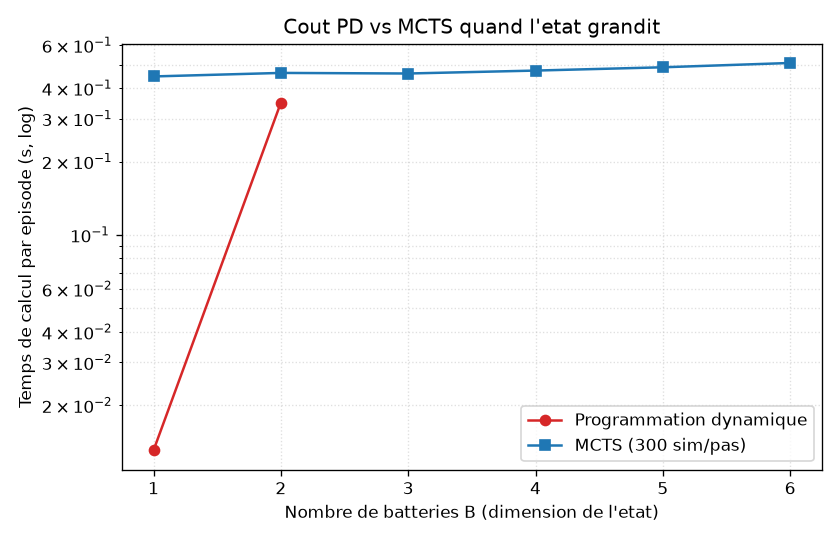
\includegraphics[width=0.72\textwidth]{../figures/scaling.png}
  \caption{Compute time per episode vs.\ number of batteries $B$ (log scale).
           DP (red) grows exponentially and crosses the almost-flat MCTS curve
           (blue) at $B=3$; beyond that, DP is infeasible while MCTS keeps
           running at the same cost.}
  \label{fig:scaling}
\end{figure}

The picture is clear. With one battery, DP is about 50 times \emph{faster}
than MCTS. But each extra battery multiplies the DP cost by roughly $n_{\soc}$,
so at $B=3$ DP already takes 13\,s (now 20 times \emph{slower} than MCTS), and
at $B=4$ the grid has 194\,481 states and DP is no longer practical. MCTS
solves all cases in well under a second, and its solution stays within about
2\% of the DP optimum wherever we can still compute it. This is the concrete
version of the ``curse of dimensionality'': DP pays for the whole state space,
MCTS only pays for the part it explores.

\subsection{Sensitivity analysis}

Figure~\ref{fig:sensitivity} shows how performance changes with the number of
simulations per step and with the exploration constant $c$, on the same
48-hour instance as Table~\ref{tab:det_results}.

\begin{figure}[H]
  \centering
  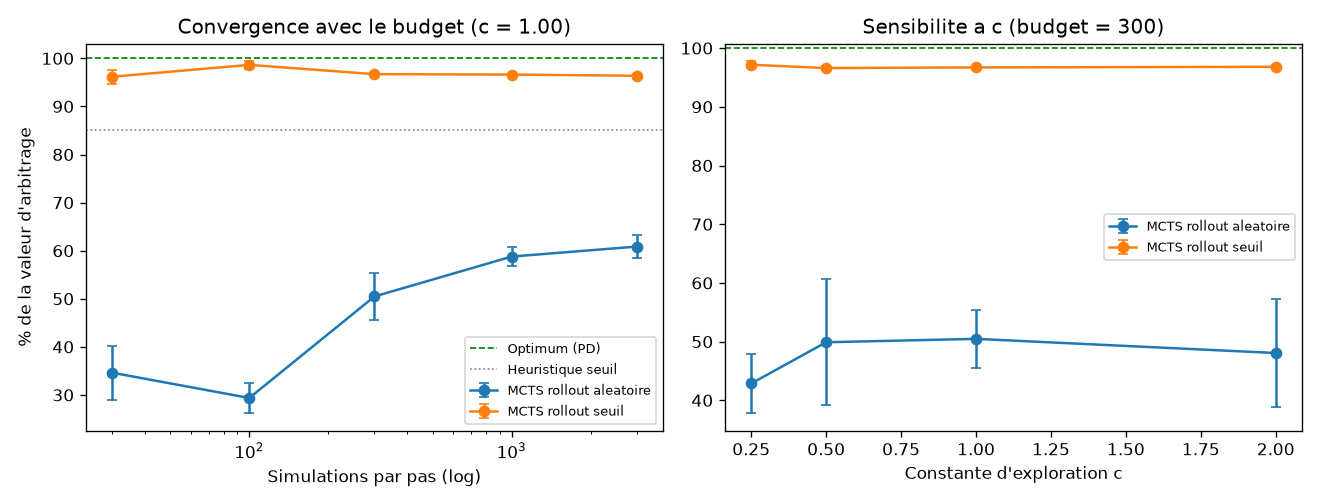
\includegraphics[width=\textwidth]{../figures/sensibilite.png}
  \caption{Left: arbitrage gain vs.\ simulation budget (log scale), with
           $c=1$, 5 seeds. Right: sensitivity to the exploration constant $c$
           at budget 300. Error bars = standard deviation. Same 48-hour
           instance as Table~\ref{tab:det_results}.}
  \label{fig:sensitivity}
\end{figure}

The key takeaway is that \textbf{the rollout is the decisive lever}:
\begin{itemize}
  \item With an \emph{informed rollout} (price threshold), MCTS is already
    excellent at every budget: about 96\% at 30 simulations per step and
    97--99\% from 100 onward. It is essentially flat, sitting just above the
    heuristic it starts from.
  \item With a \emph{random rollout}, performance climbs with the budget
    (from $\sim$35\% at 30 simulations to $\sim$61\% at 3000) but plateaus
    well below the optimum. Random continuations rarely discharge the stored
    energy at the right time, so the value estimates stay biased downward.
  \item The constant $c$ has very little effect once the rollout is
    informative (97\% across the whole range); with a random rollout the
    estimates are too noisy for $c$ to help.
\end{itemize}

Two honest remarks. First, the curves are \textbf{not perfectly monotone}:
with the informed rollout, adding more simulations can even nudge results
slightly \emph{down} (98.6\% at 100, 96.6\% at 1000), because extra
simulations pull the decision away from the already-good default rollout
toward the tree's own noisier estimates. This is expected: MCTS only converges
to the optimum in the limit of very large budgets, and here it is already near
a ceiling. Second, this near-ceiling behavior is exactly the \textbf{anytime}
property in action: you can stop early and still get a valid, near-optimal
answer.

% ==========================================================================
\section{Stochastic Extension}
% ==========================================================================

\subsection{Motivation}

In the deterministic setting, prices are known in advance (perfect
information). In practice, prices are uncertain. We now model prices as a
random process and see how well MCTS handles uncertainty.

\subsection{Price model}

We use a \textbf{Markov chain} on price deviations. The price at time $t$ is:
\begin{equation}
  \lambda_t = \max\!\bigl(\mu_t + e_t,\; \lambda_{\min}\bigr)
\end{equation}
where $\mu_t$ is a known deterministic seasonal profile (the ``duck curve''),
and $e_t$ is a stochastic deviation following a mean-reverting Markov chain
with $S = 10$ states and a fat right tail (occasional price spikes). The
transition probabilities are:
\begin{equation}
  P_{ij} \propto (1 - p_{\mathrm{spike}}) \cdot
    \exp\!\left(-\frac{(e_j - \rho\, e_i)^2}{2\sigma^2}\right)
    + p_{\mathrm{spike}} \cdot \mathbf{1}_{[j = S]}
\end{equation}
with $\rho = 0.7$ (mean reversion), $\sigma = 6$\,\euro/MWh, and
$p_{\mathrm{spike}} = 5\%$ (probability of jumping to the highest price state).

\subsection{Reference strategies}

\paragraph{Clairvoyant bound.} Run DP on the \emph{realized} price path.
This sees the future and cannot be beaten by any causal strategy.

\paragraph{Stochastic DP (SDP).} The exact causal optimum. We solve
$V(t, \soc, s) = \max_a \bigl\{ r(t, \soc, a, s) + \mathbb{E}_{s' \sim P[s]}
V(t+1, \soc', s') \bigr\}$ by backward induction on the augmented state
$(t, \soc, s)$. This is computationally feasible here (10 price states $\times$
81 SoC grid points), but becomes intractable when the price state gets richer.

\paragraph{Certainty-equivalent MPC.} At each step, replace the stochastic
price by its conditional mean, solve the deterministic DP, execute the first
action, and repeat. This is also called \emph{certainty-equivalent control}.

\paragraph{Stochastic MCTS.} Same structure as before, but after each action
we sample the next price state $s' \sim P[s]$ (instead of replaying it). The
algorithm only needs the generative model (the ability to sample $s'$), not
the full transition matrix.

\subsection{Results}

Table~\ref{tab:stoch_results} shows results averaged over 40 price scenarios
(paired evaluation: all strategies face the same scenarios).

\begin{table}[H]
  \centering
  \caption{Stochastic setting: mean profit and arbitrage gain over 40 paired
           scenarios. MCTS: 800 simulations per step.
           SDP = causal optimum (100\%). Cost of uncertainty $\approx 1\%$.}
  \label{tab:stoch_results}
  \begin{tabular}{lrrr}
    \toprule
    Strategy & Mean profit & Std & \% arbitrage (SDP = 100\%) \\
    \midrule
    Always sell                & 25\,021 & 3\,833 &   0.0\% \\
    Price threshold            & 28\,371 & 3\,242 &  83.1\% \\
    Certainty-equivalent (MPC) & 29\,038 & 3\,399 &  99.7\% \\
    MCTS, random rollout       & 25\,813 & 3\,607 &  19.7\% \\
    \textbf{MCTS, informed rollout} & 28\,648 & 3\,309 & 90.0\% \\
    SDP (causal optimum)       & 29\,050 & 3\,414 & 100.0\% \\
    \midrule
    Clairvoyant (upper bound)  & 29\,330 & --- & --- \\
    \bottomrule
  \end{tabular}
\end{table}

A few important points:
\begin{itemize}
  \item The \textbf{cost of uncertainty} (gap between clairvoyant and SDP)
    is only about 1\%. Prices are somewhat predictable here (the seasonal
    pattern dominates), so not seeing the future is not a huge disadvantage.
  \item The \textbf{certainty-equivalent MPC nearly matches the SDP} (99.7\%
    vs 100\%). Re-planning at every step effectively corrects for uncertainty.
    This is a known result for problems with low cost of uncertainty.
  \item \textbf{MCTS with informed rollout reaches 90\%} of the SDP, and this
    grows with the simulation budget. MCTS uses only the generative model
    (sampling), never the transition matrix — it would scale to richer price
    models where SDP becomes intractable.
  \item MCTS with random rollout collapses to 20\%: the stochastic setting
    makes uninformative rollouts even more harmful than in the deterministic
    case.
\end{itemize}

\textbf{A note on honesty.} MCTS does not beat the SDP here. The SDP is
optimal by construction. The value of MCTS lies in its \emph{generality}: it
can handle any generative model (learned, multi-variable, long-memory price
processes), whereas SDP requires an explicit discretized price state that
quickly becomes intractable. Once the price model grows complex enough that
SDP cannot be computed, MCTS remains applicable.

% ==========================================================================
\section{Real Data: France, June 2024}
% ==========================================================================

\subsection{Setup}

We test on a week of real French data (10--16 June 2024, 166
hours\footnote{The 7-day window is nominally 168 hours. After aligning the
price series and the solar series on their common hourly timestamps in UTC,
two boundary hours at the edges of the window do not overlap (a timezone-edge
effect between the two data sources) and are dropped, leaving 166 contiguous
hours with no internal gaps.}):
\begin{itemize}
  \item \textbf{Prices}: day-ahead market (EPEX SPOT via energy-charts.info),
    ranging from $-80$ to $+85.4$ \euro/MWh, with \textbf{20 hours of negative
    prices} caused by excess solar generation at midday.
  \item \textbf{Production}: French solar output (ODRÉ / éCO2mix, RTE), peak
    at 14\,958\,MW.
  \item \textbf{Battery}: capacity = 60\% of peak solar = 8\,975\,MWh,
    charge/discharge rates = 30\% of peak.
  \item \textbf{Internal demand}: 15\% of peak solar (2\,244\,MW constant),
    avoidance price = 90\,\euro/MWh. During hours of negative spot prices,
    consuming your own production is more profitable than selling it.
\end{itemize}

\subsection{Results}

\begin{table}[H]
  \centering
  \caption{Real data results (France, 10--16 June 2024, 166 hours).
           MCTS: 300 simulations/step, 3 seeds (mean $\pm$ std).}
  \label{tab:real_results}
  \begin{tabular}{lrrr}
    \toprule
    Strategy & Profit (\euro) & \% of optimum & \% arbitrage \\
    \midrule
    Random              & 22\,407\,778 & 81.6\% &  18.3\% \\
    No storage          & 21\,277\,253 & 77.5\% &   0.0\% \\
    Greedy-myopic       & 21\,724\,882 & 79.1\% &   7.2\% \\
    Price threshold     & 22\,841\,148 & 83.2\% &  25.3\% \\
    MCTS, random rollout & $26\,170\,455 \pm 201\,744$ & 95.3\% & 79.2\% \\
    \textbf{MCTS, informed rollout} & $\mathbf{27\,100\,439 \pm 4\,001}$ & \textbf{98.7\%} & \textbf{94.2\%} \\
    DP Optimum          & 27\,457\,018 & 100\%  & 100.0\% \\
    \bottomrule
  \end{tabular}
\end{table}

The most striking observation is how much the price-threshold heuristic
\emph{falls behind} on real data (only 25.3\% arbitrage) compared to synthetic
data (85.1\%). The reason is the \textbf{negative prices}: a fixed threshold
based on the median price does not handle them well. MCTS, which plans ahead
by simulating future states, naturally avoids selling during negative-price
hours and instead stores or consumes the energy, reaching 94.2\% of the
arbitrage value. Interestingly, even MCTS with a random rollout does well here
(79.2\%), much better than on the synthetic data: on real prices, the cost of
selling at the wrong time is so large that even noisy planning beats the fixed
heuristic.

Figure~\ref{fig:real_results} shows the real price profile (with negative-price
zones highlighted) and the storage trajectories of the main strategies.

\begin{figure}[H]
  \centering
  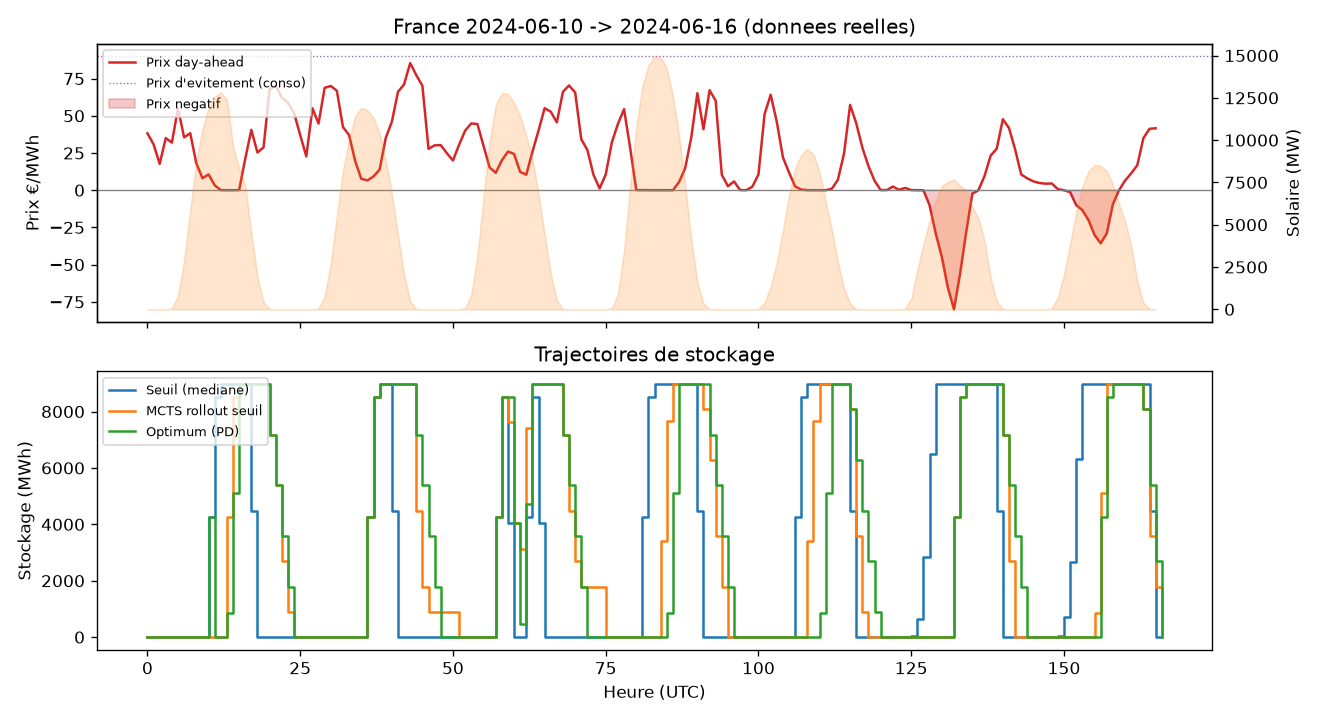
\includegraphics[width=\textwidth]{../figures/comparaison_reelle.png}
  \caption{Real French data (10--16 June 2024, 166 h). Top: day-ahead price
           (negative-price hours shaded red), solar production, and the
           avoidance price line. Bottom: storage trajectories of the threshold
           heuristic, MCTS (informed rollout), and the DP optimum. MCTS closely
           matches the optimal battery use even through the negative-price
           episodes.}
  \label{fig:real_results}
\end{figure}

% ==========================================================================
\section{Discussion}
% ==========================================================================

\subsection{Why MCTS works well here}

The energy management problem has a natural structure that suits MCTS:
\begin{enumerate}
  \item \textbf{Large action space}: $11^{H}$ or $3^{H}$ sequences are
    impossible to enumerate. MCTS focuses on the best branches.
  \item \textbf{Temporal credit assignment}: the value of storing energy now
    only appears when it is discharged later. MCTS propagates this signal
    backward through the tree.
  \item \textbf{Rollout guidance}: a simple domain heuristic (sell high, store
    low) is enough to make rollouts informative and boost performance
    dramatically.
  \item \textbf{Rolling-horizon}: re-planning at each step makes the policy
    robust, because the tree is always built from the true current state.
  \item \textbf{Scales with the state}: as shown in Section~5.4, MCTS cost
    barely grows when the state gets bigger (more batteries), while DP explodes
    exponentially. This is where MCTS earns its place.
\end{enumerate}

\subsection{Limitations and possible improvements}

\begin{itemize}
  \item \textbf{Random rollout is weak.} An uninformed rollout underestimates
    the storage value, misleads the tree, and causes slow convergence.
    This is the main weakness to address if budget is limited.
  \item \textbf{Tree reuse.} Currently, the tree is rebuilt from scratch at
    every step. Reusing the subtree rooted at the chosen action (``tree
    recycling'') would halve the effective budget needed.
  \item \textbf{Stochastic MCTS needs more budget than the deterministic
    version.} Sampling introduces variance in the value estimates, and
    convergence is slower.
  \item \textbf{The stochastic price model is simple.} A more realistic model
    (long-memory, multi-variable, learned from data) would make SDP
    intractable and give MCTS a clearer advantage over certainty-equivalent
    MPC. This is the stochastic counterpart of the scaling experiment in
    Section~5.4 (which grew the state on the deterministic side).
  \item \textbf{The consumption channel is simple here.} We used a constant
    demand and constant avoidance price. In practice, both would vary by hour,
    which would make the consume/sell trade-off more complex and further
    motivate MCTS.
\end{itemize}

% ==========================================================================
\section{Conclusion}
% ==========================================================================

We applied Monte Carlo Tree Search to an energy management problem where a
power plant must decide each hour whether to sell, store, or consume its
electricity to maximize profit.

We showed that:
\begin{itemize}
  \item MCTS with a rolling horizon is an effective planner for this type of
    problem. With an informed rollout, it captures \textbf{96.6\%} of the
    storage value on synthetic data and \textbf{94.2\%} on a real week of
    French data, reaching 98.7\% of the DP upper bound.
  \item \textbf{The rollout policy is the key design choice}: an informed
    rollout (using a simple price-threshold heuristic) makes MCTS nearly
    optimal with just 100 simulations per step; a random rollout converges
    much more slowly and plateaus well below the optimum on synthetic data
    (though it still does surprisingly well on real prices, where selling at
    the wrong time is heavily penalized).
  \item In the stochastic setting, MCTS (with informed rollout) approaches
    the exact causal optimum (SDP) using only a generative model. Its
    advantage over SDP grows as the price model becomes more complex.
  \item A subtle bug in the handling of terminal nodes (visit counting) was
    caught by unit tests and shows the importance of rigorous testing even
    for simple implementations.
\end{itemize}

Overall, MCTS is a practical and general solution for this class of problems.
Its main strength is that it only requires a simulator, not an analytical
model or an explicit transition matrix. This makes it easy to extend to richer
price models, multi-asset portfolios, or longer planning horizons, where
classical dynamic programming would quickly become intractable.

% ==========================================================================
\appendix
\section{Project Structure}
% ==========================================================================

\begin{verbatim}
Projet_MCTS/
├── core/               one implementation of everything
│   ├── environment.py  MDP simulator (sell / store / consume)
│   ├── baselines.py    reference strategies + DP optimum
│   ├── mcts.py         deterministic MCTS/UCT
│   ├── price_model.py  Markov price model
│   ├── stochastic.py   SDP, certainty-equivalent MPC, clairvoyant
│   ├── mcts_stochastic.py  stochastic MCTS
│   └── data_loader.py  real French data (EPEX + solar)
├── experiments/
│   ├── run_demo.py         deterministic demo, multi-seed
│   ├── run_sensitivity.py  budget & c sensitivity study
│   ├── run_timing.py       compute-time measurements
│   ├── run_scaling.py      DP vs MCTS scaling (multi-battery)
│   ├── run_demo_stochastic.py  stochastic Monte-Carlo evaluation
│   └── run_demo_real.py    real-data demo
├── tests/
│   └── test_core.py   15 unit tests (dynamics, DP vs brute force, MCTS)
└── figures/            generated figures
\end{verbatim}

\end{document}
